% Options for packages loaded elsewhere
\PassOptionsToPackage{unicode}{hyperref}
\PassOptionsToPackage{hyphens}{url}
\PassOptionsToPackage{dvipsnames,svgnames,x11names}{xcolor}
%
\documentclass[
  letterpaper,
  DIV=11,
  numbers=noendperiod]{scrartcl}

\usepackage{amsmath,amssymb}
\usepackage{lmodern}
\usepackage{iftex}
\ifPDFTeX
  \usepackage[T1]{fontenc}
  \usepackage[utf8]{inputenc}
  \usepackage{textcomp} % provide euro and other symbols
\else % if luatex or xetex
  \usepackage{unicode-math}
  \defaultfontfeatures{Scale=MatchLowercase}
  \defaultfontfeatures[\rmfamily]{Ligatures=TeX,Scale=1}
\fi
% Use upquote if available, for straight quotes in verbatim environments
\IfFileExists{upquote.sty}{\usepackage{upquote}}{}
\IfFileExists{microtype.sty}{% use microtype if available
  \usepackage[]{microtype}
  \UseMicrotypeSet[protrusion]{basicmath} % disable protrusion for tt fonts
}{}
\makeatletter
\@ifundefined{KOMAClassName}{% if non-KOMA class
  \IfFileExists{parskip.sty}{%
    \usepackage{parskip}
  }{% else
    \setlength{\parindent}{0pt}
    \setlength{\parskip}{6pt plus 2pt minus 1pt}}
}{% if KOMA class
  \KOMAoptions{parskip=half}}
\makeatother
\usepackage{xcolor}
\setlength{\emergencystretch}{3em} % prevent overfull lines
\setcounter{secnumdepth}{-\maxdimen} % remove section numbering
% Make \paragraph and \subparagraph free-standing
\ifx\paragraph\undefined\else
  \let\oldparagraph\paragraph
  \renewcommand{\paragraph}[1]{\oldparagraph{#1}\mbox{}}
\fi
\ifx\subparagraph\undefined\else
  \let\oldsubparagraph\subparagraph
  \renewcommand{\subparagraph}[1]{\oldsubparagraph{#1}\mbox{}}
\fi

\usepackage{color}
\usepackage{fancyvrb}
\newcommand{\VerbBar}{|}
\newcommand{\VERB}{\Verb[commandchars=\\\{\}]}
\DefineVerbatimEnvironment{Highlighting}{Verbatim}{commandchars=\\\{\}}
% Add ',fontsize=\small' for more characters per line
\usepackage{framed}
\definecolor{shadecolor}{RGB}{241,243,245}
\newenvironment{Shaded}{\begin{snugshade}}{\end{snugshade}}
\newcommand{\AlertTok}[1]{\textcolor[rgb]{0.68,0.00,0.00}{#1}}
\newcommand{\AnnotationTok}[1]{\textcolor[rgb]{0.37,0.37,0.37}{#1}}
\newcommand{\AttributeTok}[1]{\textcolor[rgb]{0.40,0.45,0.13}{#1}}
\newcommand{\BaseNTok}[1]{\textcolor[rgb]{0.68,0.00,0.00}{#1}}
\newcommand{\BuiltInTok}[1]{\textcolor[rgb]{0.00,0.23,0.31}{#1}}
\newcommand{\CharTok}[1]{\textcolor[rgb]{0.13,0.47,0.30}{#1}}
\newcommand{\CommentTok}[1]{\textcolor[rgb]{0.37,0.37,0.37}{#1}}
\newcommand{\CommentVarTok}[1]{\textcolor[rgb]{0.37,0.37,0.37}{\textit{#1}}}
\newcommand{\ConstantTok}[1]{\textcolor[rgb]{0.56,0.35,0.01}{#1}}
\newcommand{\ControlFlowTok}[1]{\textcolor[rgb]{0.00,0.23,0.31}{#1}}
\newcommand{\DataTypeTok}[1]{\textcolor[rgb]{0.68,0.00,0.00}{#1}}
\newcommand{\DecValTok}[1]{\textcolor[rgb]{0.68,0.00,0.00}{#1}}
\newcommand{\DocumentationTok}[1]{\textcolor[rgb]{0.37,0.37,0.37}{\textit{#1}}}
\newcommand{\ErrorTok}[1]{\textcolor[rgb]{0.68,0.00,0.00}{#1}}
\newcommand{\ExtensionTok}[1]{\textcolor[rgb]{0.00,0.23,0.31}{#1}}
\newcommand{\FloatTok}[1]{\textcolor[rgb]{0.68,0.00,0.00}{#1}}
\newcommand{\FunctionTok}[1]{\textcolor[rgb]{0.28,0.35,0.67}{#1}}
\newcommand{\ImportTok}[1]{\textcolor[rgb]{0.00,0.46,0.62}{#1}}
\newcommand{\InformationTok}[1]{\textcolor[rgb]{0.37,0.37,0.37}{#1}}
\newcommand{\KeywordTok}[1]{\textcolor[rgb]{0.00,0.23,0.31}{#1}}
\newcommand{\NormalTok}[1]{\textcolor[rgb]{0.00,0.23,0.31}{#1}}
\newcommand{\OperatorTok}[1]{\textcolor[rgb]{0.37,0.37,0.37}{#1}}
\newcommand{\OtherTok}[1]{\textcolor[rgb]{0.00,0.23,0.31}{#1}}
\newcommand{\PreprocessorTok}[1]{\textcolor[rgb]{0.68,0.00,0.00}{#1}}
\newcommand{\RegionMarkerTok}[1]{\textcolor[rgb]{0.00,0.23,0.31}{#1}}
\newcommand{\SpecialCharTok}[1]{\textcolor[rgb]{0.37,0.37,0.37}{#1}}
\newcommand{\SpecialStringTok}[1]{\textcolor[rgb]{0.13,0.47,0.30}{#1}}
\newcommand{\StringTok}[1]{\textcolor[rgb]{0.13,0.47,0.30}{#1}}
\newcommand{\VariableTok}[1]{\textcolor[rgb]{0.07,0.07,0.07}{#1}}
\newcommand{\VerbatimStringTok}[1]{\textcolor[rgb]{0.13,0.47,0.30}{#1}}
\newcommand{\WarningTok}[1]{\textcolor[rgb]{0.37,0.37,0.37}{\textit{#1}}}

\providecommand{\tightlist}{%
  \setlength{\itemsep}{0pt}\setlength{\parskip}{0pt}}\usepackage{longtable,booktabs,array}
\usepackage{calc} % for calculating minipage widths
% Correct order of tables after \paragraph or \subparagraph
\usepackage{etoolbox}
\makeatletter
\patchcmd\longtable{\par}{\if@noskipsec\mbox{}\fi\par}{}{}
\makeatother
% Allow footnotes in longtable head/foot
\IfFileExists{footnotehyper.sty}{\usepackage{footnotehyper}}{\usepackage{footnote}}
\makesavenoteenv{longtable}
\usepackage{graphicx}
\makeatletter
\def\maxwidth{\ifdim\Gin@nat@width>\linewidth\linewidth\else\Gin@nat@width\fi}
\def\maxheight{\ifdim\Gin@nat@height>\textheight\textheight\else\Gin@nat@height\fi}
\makeatother
% Scale images if necessary, so that they will not overflow the page
% margins by default, and it is still possible to overwrite the defaults
% using explicit options in \includegraphics[width, height, ...]{}
\setkeys{Gin}{width=\maxwidth,height=\maxheight,keepaspectratio}
% Set default figure placement to htbp
\makeatletter
\def\fps@figure{htbp}
\makeatother

\usepackage{booktabs}
\usepackage{longtable}
\usepackage{array}
\usepackage{multirow}
\usepackage{wrapfig}
\usepackage{float}
\usepackage{colortbl}
\usepackage{pdflscape}
\usepackage{tabu}
\usepackage{threeparttable}
\usepackage{threeparttablex}
\usepackage[normalem]{ulem}
\usepackage{makecell}
\usepackage{xcolor}
\usepackage[auth-lg]{authblk}
\setlength{\parindent}{20pt}
\KOMAoption{captions}{tableheading}
\makeatletter
\makeatother
\makeatletter
\makeatother
\makeatletter
\@ifpackageloaded{caption}{}{\usepackage{caption}}
\AtBeginDocument{%
\ifdefined\contentsname
  \renewcommand*\contentsname{Table of contents}
\else
  \newcommand\contentsname{Table of contents}
\fi
\ifdefined\listfigurename
  \renewcommand*\listfigurename{List of Figures}
\else
  \newcommand\listfigurename{List of Figures}
\fi
\ifdefined\listtablename
  \renewcommand*\listtablename{List of Tables}
\else
  \newcommand\listtablename{List of Tables}
\fi
\ifdefined\figurename
  \renewcommand*\figurename{Figure}
\else
  \newcommand\figurename{Figure}
\fi
\ifdefined\tablename
  \renewcommand*\tablename{Table}
\else
  \newcommand\tablename{Table}
\fi
}
\@ifpackageloaded{float}{}{\usepackage{float}}
\floatstyle{ruled}
\@ifundefined{c@chapter}{\newfloat{codelisting}{h}{lop}}{\newfloat{codelisting}{h}{lop}[chapter]}
\floatname{codelisting}{Listing}
\newcommand*\listoflistings{\listof{codelisting}{List of Listings}}
\makeatother
\makeatletter
\@ifpackageloaded{caption}{}{\usepackage{caption}}
\@ifpackageloaded{subcaption}{}{\usepackage{subcaption}}
\makeatother
\makeatletter
\@ifpackageloaded{tcolorbox}{}{\usepackage[many]{tcolorbox}}
\makeatother
\makeatletter
\@ifundefined{shadecolor}{\definecolor{shadecolor}{rgb}{.97, .97, .97}}
\makeatother
\makeatletter
\makeatother
\ifLuaTeX
  \usepackage{selnolig}  % disable illegal ligatures
\fi
\IfFileExists{bookmark.sty}{\usepackage{bookmark}}{\usepackage{hyperref}}
\IfFileExists{xurl.sty}{\usepackage{xurl}}{} % add URL line breaks if available
\urlstyle{same} % disable monospaced font for URLs
\hypersetup{
  pdftitle={Trabalho Prático 1},
  pdfauthor={Carolina Musso 18/0047850; Gabriela Carneiro de Almeida 18/0120816; Renan Menezes de Araujo},
  colorlinks=true,
  linkcolor={blue},
  filecolor={Maroon},
  citecolor={Blue},
  urlcolor={Blue},
  pdfcreator={LaTeX via pandoc}}

\title{Trabalho Prático 1}
\usepackage{etoolbox}
\makeatletter
\providecommand{\subtitle}[1]{% add subtitle to \maketitle
  \apptocmd{\@title}{\par {\large #1 \par}}{}{}
}
\makeatother
\subtitle{Séries Temporais - 1/2023}
\author{Carolina Musso 18/0047850 \and Gabriela Carneiro de Almeida
18/0120816 \and Renan Menezes de Araujo}
\date{}

\begin{document}
\maketitle
\ifdefined\Shaded\renewenvironment{Shaded}{\begin{tcolorbox}[enhanced, sharp corners, interior hidden, breakable, boxrule=0pt, borderline west={3pt}{0pt}{shadecolor}, frame hidden]}{\end{tcolorbox}}\fi

\renewcommand*\contentsname{Table of contents}
{
\hypersetup{linkcolor=}
\setcounter{tocdepth}{3}
\tableofcontents
}
\newpage{}

\hypertarget{introduuxe7uxe3o}{%
\section{Introdução}\label{introduuxe7uxe3o}}

\begin{Shaded}
\begin{Highlighting}[]
\NormalTok{pacman}\SpecialCharTok{::}\FunctionTok{p\_load}\NormalTok{(Mcomp, tidyverse, forecast, flextable)}
\end{Highlighting}
\end{Shaded}

O pacote Mcomp disponibiliza milhares de séries de competições de
previsão de séries temporais. A série apresentada nesse trabalho é a de
id 2342, que se refe a uma pesquisa sobre ``Manufacturers' shipments,
paper and allied products'', da comepetição M3. Ela fornece dados
estatísticos mensais sobre as condições econômicas no setor de
manufatura doméstica (empresas pequenas). A pesquisa mensura a atividade
industrial atual e fornece uma indicação das tendências futuras desses
tipos de negócios. Essa série mensal apresenta dados observados de
Janeiro de 1983 a Agosto de 1992, e um horizonte de previsão de 18,
projetando os resultados até Fevereiro de 1994.

Abaixo podemos observar os dados fornecidos nessa série, bem como seu
gráfico, onde o horizonte de previsão aparece em vermelho.

\begin{Shaded}
\begin{Highlighting}[]
\FunctionTok{data}\NormalTok{(M3)}
\NormalTok{id1 }\OtherTok{\textless{}{-}} \DecValTok{2342} 
\CommentTok{\#id2 \textless{}{-} 1965}

\NormalTok{serie }\OtherTok{\textless{}{-}}\NormalTok{ M3[[id1]] }\CommentTok{\# serie}
\NormalTok{serie}
\end{Highlighting}
\end{Shaded}

\begin{verbatim}
Series: M941
Type of series: MACRO
Period of series: MONTHLY
Series description: Manufacturers' shipments, paper and allied products

HISTORICAL data
        Jan    Feb    Mar    Apr    May    Jun    Jul    Aug    Sep    Oct
1983 3281.0 3397.0 3498.5 3538.0 3449.5 3673.0 3350.5 3604.0 3673.5 3747.0
1984 3710.0 3994.5 4091.0 3954.5 4004.0 4287.0 3831.0 4046.5 4079.5 4029.5
1985 3841.5 4123.5 4133.0 3958.5 4003.0 4151.5 3723.0 3957.0 3965.5 3861.5
1986 3950.0 4140.5 4090.0 4162.0 4066.0 4358.5 4022.5 4285.5 4373.5 4284.5
1987 4181.5 4535.5 4497.0 4420.5 4370.0 4712.0 4475.0 4578.5 4751.5 4746.0
1988 4751.0 4952.5 4996.5 4998.0 4986.5 5348.0 4933.0 5263.0 5330.5 5301.0
1989 5411.5 5536.5 5613.0 5505.5 5476.0 5782.5 5283.0 5451.5 5578.0 5548.5
1990 5316.5 5505.5 5620.5 5383.5 5461.5 5658.5 5357.5 5622.0 5608.0 5604.5
1991 5221.0 5379.5 5333.0 5214.0 5206.5 5630.0 5285.5 5512.5 5592.5 5554.5
1992 5241.5 5455.0 5548.5 5375.0 5346.0 5730.5 5457.0 5603.0              
        Nov    Dec
1983 3616.0 3580.5
1984 3880.0 3855.0
1985 3917.5 3704.0
1986 4077.5 4122.0
1987 4581.5 4645.5
1988 5159.0 5258.5
1989 5379.5 5117.5
1990 5399.0 5185.0
1991 5284.5 5198.5
1992              

FUTURE data
        Jan    Feb    Mar    Apr    May    Jun    Jul    Aug    Sep    Oct
1992                                                         5628.5 5515.0
1993 5274.0 5382.5 5503.5 5146.5 5364.0 5608.0 5280.5 5432.5 5636.5 5442.5
1994 5114.0 5429.5                                                        
        Nov    Dec
1992 5378.0 5375.5
1993 5321.0 5195.5
1994              
\end{verbatim}

\begin{Shaded}
\begin{Highlighting}[]
\FunctionTok{plot}\NormalTok{(serie)}
\end{Highlighting}
\end{Shaded}

\begin{figure}[H]

{\centering 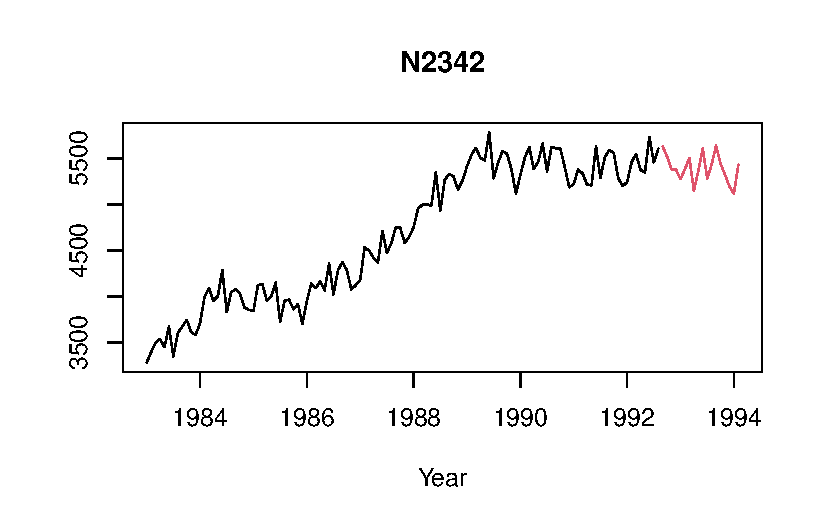
\includegraphics{Trabalhao1_ST_grupo5_2023_05_16_files/figure-pdf/figura-1.pdf}

}

\caption{Série 2342}

\end{figure}

\hypertarget{a.-decomposiuxe7uxe3o-da-suxe9rie-temporal-via-stl-ou-mstl.}{%
\subsection{a. Decomposição da série temporal via STL (ou
MSTL).}\label{a.-decomposiuxe7uxe3o-da-suxe9rie-temporal-via-stl-ou-mstl.}}

\begin{Shaded}
\begin{Highlighting}[]
\CommentTok{\# obtendo os dados observados}

\NormalTok{dados }\OtherTok{\textless{}{-}}\NormalTok{ serie}\SpecialCharTok{$}\NormalTok{x}

\NormalTok{dados }\SpecialCharTok{\%\textgreater{}\%} \FunctionTok{stl}\NormalTok{(}\AttributeTok{s.window =} \DecValTok{7}\NormalTok{) }\SpecialCharTok{\%\textgreater{}\%}
  \FunctionTok{plot}\NormalTok{()}
\end{Highlighting}
\end{Shaded}

\begin{figure}[H]

{\centering 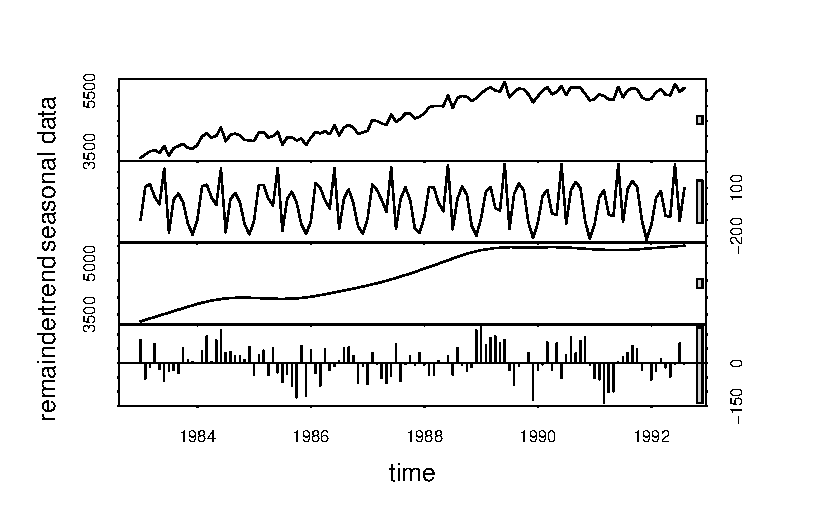
\includegraphics{Trabalhao1_ST_grupo5_2023_05_16_files/figure-pdf/unnamed-chunk-3-1.pdf}

}

\end{figure}

Primeiramente, a função stl() - ``Seasonal an trending using Loess''-
foi utilizada para decompor a série analisada com o parâmetro s.window
(janela sazonal) configurado para 7, como é recomendado por Cleveland et
al.~(1990).

No caso específico dessa série, ela já não aparentava ter comportamentos
sazonais dinâmicos muito expressivos. Assim, ao usar a função stl() com
o parâmetro de janela ``periodic'' (para utilizar a média) ou
simplesmente utilizando uma decomposição aditiva clássica da função
\texttt{decompose()}, a tendência e parâmetro sazonais já estavam sendo
capturados de forma clara.

Entretanto, apesar de ter sido observado que a partir dessa janela
sazonal o comportamento dos resíduos já melhorava (em contraste com
janelas de 3, ou 5), ainda consideramos que havia um pouco de
comportamento sazonal restante nos erros. Por esse motivo foram
experimentados outros tamanhos de janela de tendência, chegando-se a um
valor ideal de t.window=7.

\begin{Shaded}
\begin{Highlighting}[]
\NormalTok{dados }\SpecialCharTok{\%\textgreater{}\%} \FunctionTok{stl}\NormalTok{(}\AttributeTok{s.window =} \DecValTok{7}\NormalTok{, }\AttributeTok{t.window =}\DecValTok{7}\NormalTok{) }\SpecialCharTok{\%\textgreater{}\%}
  \FunctionTok{plot}\NormalTok{()}
\end{Highlighting}
\end{Shaded}

\begin{figure}[H]

{\centering 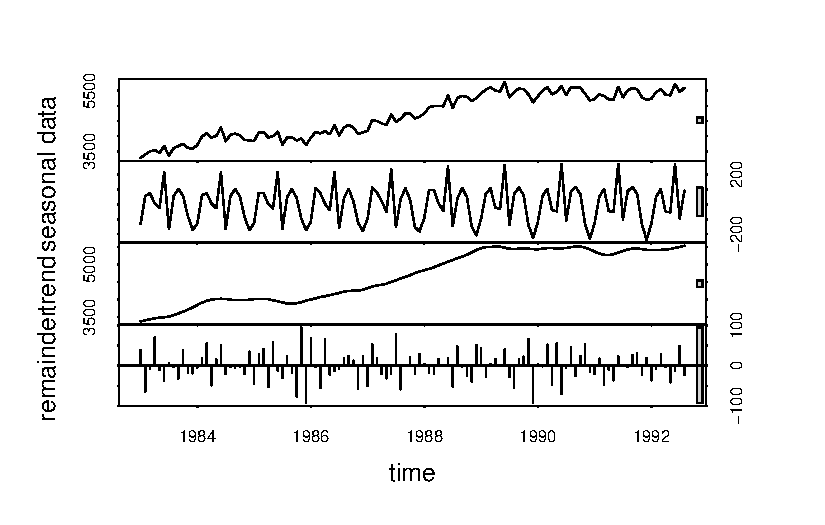
\includegraphics{Trabalhao1_ST_grupo5_2023_05_16_files/figure-pdf/unnamed-chunk-4-1.pdf}

}

\end{figure}

Agora, consideramos que os resíduos estão mais bem comportados em
relação à decompsição anterior. Agora notamos uma pequena dinamicidade
nos termos sazonais, sendo que os termos mais recentes tem uma amplitude
levemente maior.

Como pode ser observado no gráfico, há uma tendência crescente clara na
série, seguido de um platô a partir de 1990, já observável mesmo antes
da decomposição. Uma vez que vamos considerar esses resíduos da última
decompsição como compatíveis a um ruido branco, vemos que o componente
de tendência foi bem capturado pela decomposição.

Há também um padrão sazonal anual na série, aque apresenta três picos a
cada ano e, como dito anteriormente, parece apresentar um leve aumento
na amplitude para os anos mais recentes.

Uma alternativa à função stl() seria a função mstl(), que aplica o mesmo
método de forma automatizada, ou seja, sem a necessidade de setar
previamente o tamanho da janela sazonal. Apesar de ele também
automaticamente sugerir um tamanho para t.window(), consideramos que o
melhor resultado surgiu quando ele também foi configurado manualmente
para \texttt{t.window=\ 7}, como discutimos anteriormente. Outra
vantagem da função mstl() é que ela seria capaz de identificar multiplas
sazonalidades, caso ocorressem.

\begin{Shaded}
\begin{Highlighting}[]
\NormalTok{dados }\SpecialCharTok{\%\textgreater{}\%} \FunctionTok{mstl}\NormalTok{(}\AttributeTok{lambda =} \StringTok{"auto"}\NormalTok{, }\AttributeTok{t.window=}\DecValTok{7}\NormalTok{ ) }\SpecialCharTok{\%\textgreater{}\%}\NormalTok{ plot}
\end{Highlighting}
\end{Shaded}

\begin{figure}[H]

{\centering 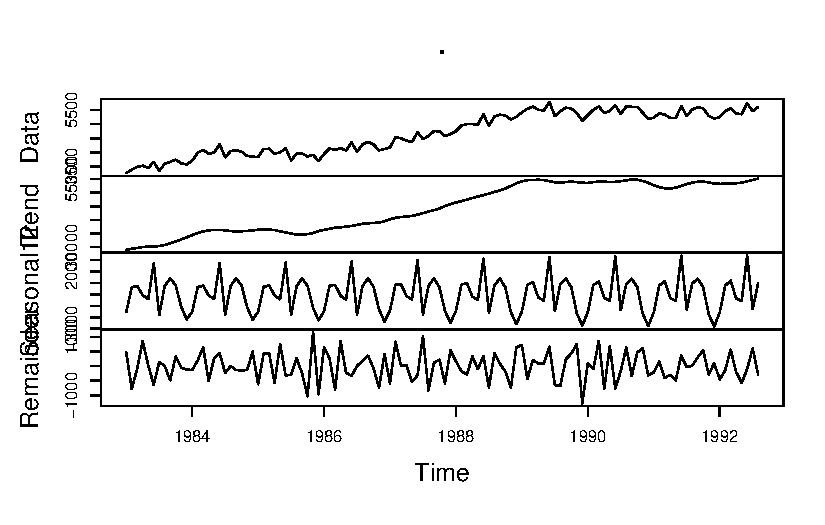
\includegraphics{Trabalhao1_ST_grupo5_2023_05_16_files/figure-pdf/unnamed-chunk-5-1.pdf}

}

\end{figure}

O gráfico da decomposição MSTL indicou que não há multiplas
sazonalidades, estando compatível com as interpretações já apresentadas
acima.

\hypertarget{b.-escolha-um-modelo-arima-adequado-de-forma-manual.}{%
\subsection{b. Escolha um modelo ARIMA adequado de forma
manual.}\label{b.-escolha-um-modelo-arima-adequado-de-forma-manual.}}

Primeiramente, vamos verificar se há necessidade de difenciações simples
ou sazonais. Aplicando a função ndiffs() encontramos a necessidade de:

\begin{Shaded}
\begin{Highlighting}[]
\NormalTok{dados }\SpecialCharTok{\%\textgreater{}\%} \FunctionTok{ndiffs}\NormalTok{() }
\end{Highlighting}
\end{Shaded}

\begin{verbatim}
[1] 1
\end{verbatim}

Observando o gráfico após essa diferenciação simples:

\begin{Shaded}
\begin{Highlighting}[]
\NormalTok{dif\_simples }\OtherTok{\textless{}{-}}\NormalTok{ dados }\SpecialCharTok{\%\textgreater{}\%} \FunctionTok{diff}\NormalTok{() }

\FunctionTok{par}\NormalTok{(}\AttributeTok{mfrow=}\FunctionTok{c}\NormalTok{(}\DecValTok{1}\NormalTok{,}\DecValTok{3}\NormalTok{))}
\FunctionTok{plot}\NormalTok{(dif\_simples )}
\FunctionTok{acf}\NormalTok{(dif\_simples , }\AttributeTok{lag.max =} \DecValTok{12}\SpecialCharTok{*}\DecValTok{4}\NormalTok{)}
\FunctionTok{pacf}\NormalTok{(dif\_simples , }\AttributeTok{lag.max =} \DecValTok{12}\SpecialCharTok{*}\DecValTok{4}\NormalTok{)}
\end{Highlighting}
\end{Shaded}

\begin{figure}[H]

{\centering 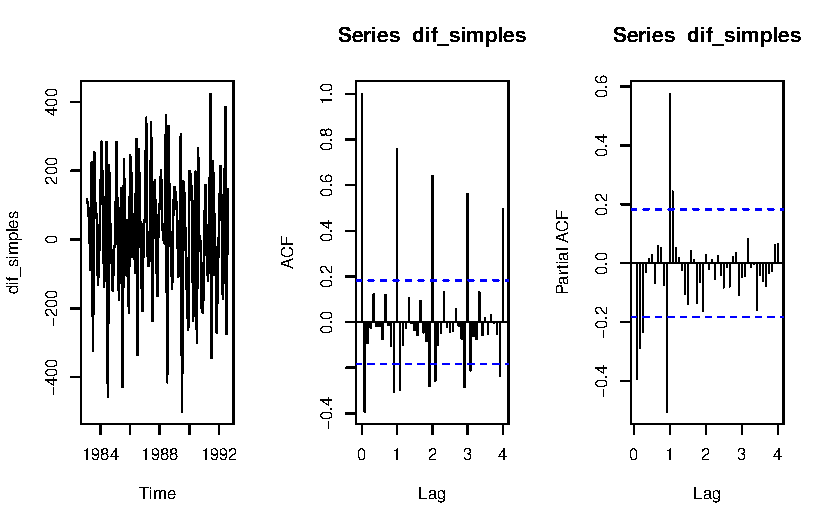
\includegraphics{Trabalhao1_ST_grupo5_2023_05_16_files/figure-pdf/unnamed-chunk-7-1.pdf}

}

\end{figure}

Notamos que após essaa diferenciação simples ainda há evidência de muita
autocorrelação nos termos sazonais.

Ou seja, o modelo ainda não é estacionário, e não podemos analisar esses
gráficos para encontrar a ordem do modelo. Assim, procede-se com a busca
pelo número de diferenciações necessárias.

\begin{Shaded}
\begin{Highlighting}[]
\NormalTok{dif\_sazonal }\OtherTok{\textless{}{-}}\NormalTok{ dif\_simples }\SpecialCharTok{\%\textgreater{}\%} \FunctionTok{nsdiffs}\NormalTok{()}
\NormalTok{dif\_sazonal}
\end{Highlighting}
\end{Shaded}

\begin{verbatim}
[1] 1
\end{verbatim}

Resumindo então, conforme observado na tabela abaixo, a série se torna
estacionária com um diferenciação simples e necessita, também, de uma
diferenciação sazonal.

\begin{Shaded}
\begin{Highlighting}[]
\NormalTok{tabela }\OtherTok{\textless{}{-}} \FunctionTok{tibble}\NormalTok{(}
  \AttributeTok{var1 =}\NormalTok{ dados }\SpecialCharTok{\%\textgreater{}\%} \FunctionTok{ndiffs}\NormalTok{(),}
  \AttributeTok{var2 =}\NormalTok{ dados }\SpecialCharTok{\%\textgreater{}\%} \FunctionTok{diff}\NormalTok{() }\SpecialCharTok{\%\textgreater{}\%} \FunctionTok{nsdiffs}\NormalTok{()}

\NormalTok{)}

\NormalTok{tabela }\SpecialCharTok{\%\textgreater{}\%}
\NormalTok{  knitr}\SpecialCharTok{::}\FunctionTok{kable}\NormalTok{(}
    \AttributeTok{format =} \StringTok{"latex"}\NormalTok{,}
    \AttributeTok{align =} \StringTok{"c"}\NormalTok{,}
    \AttributeTok{booktabs =} \ConstantTok{TRUE}\NormalTok{,}
    \AttributeTok{longtable =} \ConstantTok{TRUE}\NormalTok{,}
    \AttributeTok{linesep =} \StringTok{""}\NormalTok{,}
    \AttributeTok{col.names =} \FunctionTok{c}\NormalTok{(}\StringTok{"Número de diferenciações simples (d)"}\NormalTok{, }\StringTok{"Número de diferenciações sazonais (D)"}\NormalTok{),}
\NormalTok{    ) }\SpecialCharTok{\%\textgreater{}\%}
\NormalTok{  kableExtra}\SpecialCharTok{::}\FunctionTok{kable\_styling}\NormalTok{(}
      \AttributeTok{position =} \StringTok{"center"}\NormalTok{,}
      \AttributeTok{latex\_options =} \FunctionTok{c}\NormalTok{(}\StringTok{"striped"}\NormalTok{, }\StringTok{"repeat\_header"}\NormalTok{),}
      \AttributeTok{stripe\_color =} \StringTok{"gray!15"}\NormalTok{)}
\end{Highlighting}
\end{Shaded}

\begin{longtable}{cc}
\toprule
Número de diferenciações simples (d) & Número de diferenciações sazonais (D)\\
\midrule
\endfirsthead
\multicolumn{2}{@{}l}{\textit{(continued)}}\\
\toprule
Número de diferenciações simples (d) & Número de diferenciações sazonais (D)\\
\midrule
\endhead

\endfoot
\bottomrule
\endlastfoot
\cellcolor{gray!15}{1} & \cellcolor{gray!15}{1}\\*
\end{longtable}

Assim, a séria seguiria um modelo:

\begin{align*}
  SARIMA (p, 1, q) X (P, 1, Q)
\end{align*}

Aplicando então as diferenciações necessárias, podemos agora prosseguir
com a análise dos gráficos ACF e PACF.

\begin{Shaded}
\begin{Highlighting}[]
\NormalTok{m }\OtherTok{\textless{}{-}}\NormalTok{ dados }\SpecialCharTok{\%\textgreater{}\%} \FunctionTok{diff}\NormalTok{() }\SpecialCharTok{\%\textgreater{}\%} \FunctionTok{diff}\NormalTok{(}\AttributeTok{lag =} \DecValTok{12}\NormalTok{)}
\FunctionTok{par}\NormalTok{(}\AttributeTok{mfrow=}\FunctionTok{c}\NormalTok{(}\DecValTok{1}\NormalTok{,}\DecValTok{3}\NormalTok{))}
\FunctionTok{plot}\NormalTok{(m)}
\FunctionTok{acf}\NormalTok{(m, }\AttributeTok{lag.max =} \DecValTok{12}\SpecialCharTok{*}\DecValTok{4}\NormalTok{)}
\FunctionTok{pacf}\NormalTok{(m, }\AttributeTok{lag.max =} \DecValTok{12}\SpecialCharTok{*}\DecValTok{4}\NormalTok{)}
\end{Highlighting}
\end{Shaded}

\begin{figure}[H]

{\centering 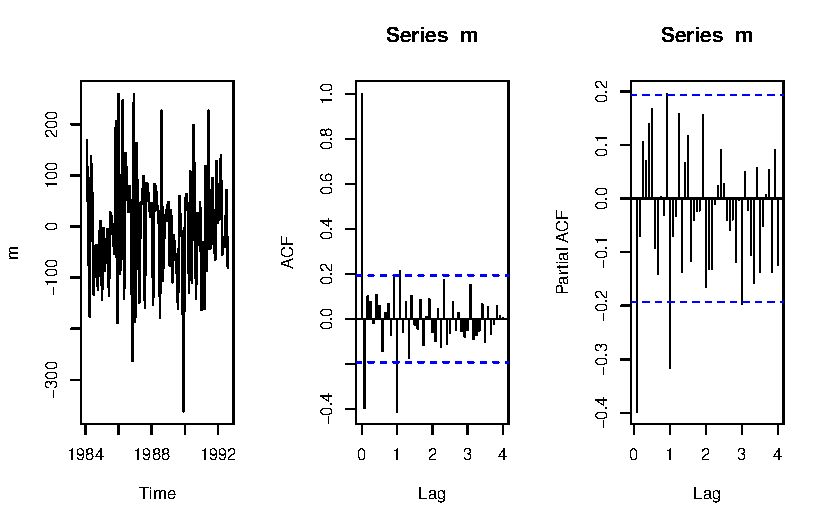
\includegraphics{Trabalhao1_ST_grupo5_2023_05_16_files/figure-pdf/unnamed-chunk-10-1.pdf}

}

\end{figure}

Olhando primeiramente os termos sazonais, eles parecem ter uma quebra na
ordem 1 no ACF e um decaimento mais amortizado no PACF, o que
caracterizaria um padrão de médias móveis para o modelo sazonal, ou seja
com P=0, 1, Q=1.

Já a parte simples parece também seguir um padrão mais póximo ao MA (em
comparação a um AR ou ARMA). Entretanto o padrão das quebras e
decaimentos não está muito claro. Por esse motivo, para a busca do
melhor modelo vamos fixar, d, D, P e Q mas vamos testar valores para p e
q.

Testamos então combinações de p e q variando de 0 a 3.

\begin{Shaded}
\begin{Highlighting}[]
\NormalTok{melhor\_AICc }\OtherTok{=} \ConstantTok{Inf}
\ControlFlowTok{for}\NormalTok{(p }\ControlFlowTok{in} \DecValTok{0}\SpecialCharTok{:}\DecValTok{3}\NormalTok{)\{}
  \ControlFlowTok{for}\NormalTok{(q }\ControlFlowTok{in} \DecValTok{0}\SpecialCharTok{:}\DecValTok{3}\NormalTok{)\{}
\NormalTok{    fit }\OtherTok{=} \FunctionTok{Arima}\NormalTok{(dados,}\AttributeTok{order=}\FunctionTok{c}\NormalTok{(p,}\DecValTok{1}\NormalTok{,q),}\AttributeTok{seasonal=}\FunctionTok{c}\NormalTok{(}\DecValTok{0}\NormalTok{,}\DecValTok{1}\NormalTok{,}\DecValTok{1}\NormalTok{))}
    \ControlFlowTok{if}\NormalTok{(fit}\SpecialCharTok{$}\NormalTok{aicc }\SpecialCharTok{\textless{}}\NormalTok{ melhor\_AICc)\{}
\NormalTok{      melhor\_AICc }\OtherTok{=}\NormalTok{ fit}\SpecialCharTok{$}\NormalTok{aicc}
      \FunctionTok{cat}\NormalTok{(}\StringTok{"p ="}\NormalTok{,p,}\StringTok{", q ="}\NormalTok{,q,}\StringTok{", AICc ="}\NormalTok{, fit}\SpecialCharTok{$}\NormalTok{aicc, }\StringTok{"}\SpecialCharTok{\textbackslash{}n}\StringTok{"}\NormalTok{)}
\NormalTok{    \}}
\NormalTok{  \}}
\NormalTok{\}}
\end{Highlighting}
\end{Shaded}

\begin{verbatim}
p = 0 , q = 0 , AICc = 1231.266 
p = 0 , q = 1 , AICc = 1225.773 
p = 0 , q = 2 , AICc = 1224.901 
p = 0 , q = 3 , AICc = 1224.69 
p = 1 , q = 0 , AICc = 1224.411 
\end{verbatim}

Melhor menor valor do critério de informação de Akaike encontrado foi
paraapresentado para a p=0 e q=2. Assim, o modelo escolhido é:

\begin{align*}
  SARIMA (0, 1, 2) X (0, 1, 1)
\end{align*}

que apresentou o AIC corrigido de 1144,458.

Procedemos então com o ajuste do modelo selecionado para obtenção dos
parâmetros.

\begin{Shaded}
\begin{Highlighting}[]
\NormalTok{fit }\OtherTok{=} \FunctionTok{Arima}\NormalTok{(dados, }\AttributeTok{order =} \FunctionTok{c}\NormalTok{(}\DecValTok{0}\NormalTok{,}\DecValTok{1}\NormalTok{,}\DecValTok{2}\NormalTok{), }\AttributeTok{seasonal =} \FunctionTok{c}\NormalTok{(}\DecValTok{0}\NormalTok{,}\DecValTok{1}\NormalTok{,}\DecValTok{1}\NormalTok{))}
\NormalTok{fit}
\end{Highlighting}
\end{Shaded}

\begin{verbatim}
Series: dados 
ARIMA(0,1,2)(0,1,1)[12] 

Coefficients:
          ma1     ma2     sma1
      -0.3468  0.1799  -0.7813
s.e.   0.1095  0.0985   0.1238

sigma^2 = 7275:  log likelihood = -608.25
AIC=1224.49   AICc=1224.9   BIC=1235.03
\end{verbatim}

\hypertarget{c.-anuxe1lise-de-resuxedduos-do-modelo-selecionado.}{%
\subsection{c.~Análise de resíduos do modelo
selecionado.}\label{c.-anuxe1lise-de-resuxedduos-do-modelo-selecionado.}}

\begin{Shaded}
\begin{Highlighting}[]
\NormalTok{E1 }\OtherTok{\textless{}{-}}\NormalTok{ fit}\SpecialCharTok{$}\NormalTok{residuals}
\FunctionTok{plot}\NormalTok{(E1);}\CommentTok{\# resíduos com zeros na inicialização}
\end{Highlighting}
\end{Shaded}

\begin{figure}[H]

{\centering 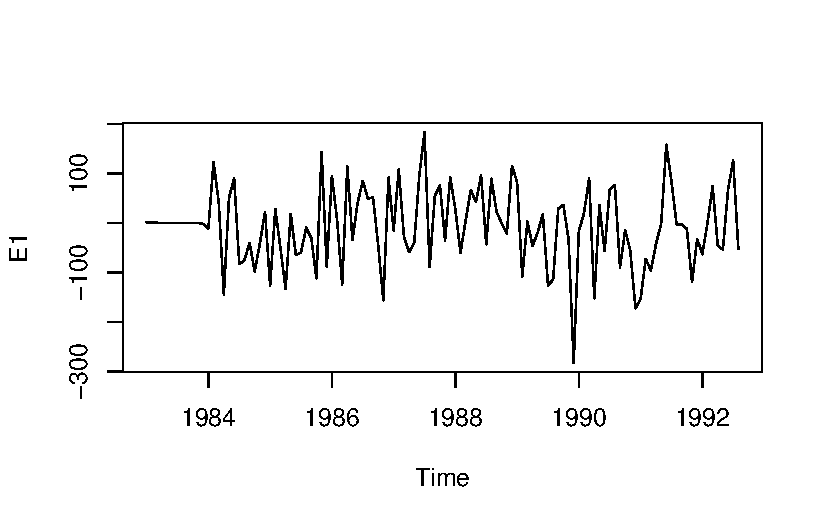
\includegraphics{Trabalhao1_ST_grupo5_2023_05_16_files/figure-pdf/unnamed-chunk-13-1.pdf}

}

\end{figure}

Por ser um modelo que requer diferenciação, nota-se que perdemos as
primeiras observações dos resíduos para a inicialização. Assim, vamos
analizar os resíduos após a remoção dessa primeira parte de zeros.

\begin{Shaded}
\begin{Highlighting}[]
\NormalTok{E }\OtherTok{\textless{}{-}}\NormalTok{ fit}\SpecialCharTok{$}\NormalTok{residuals }\SpecialCharTok{\%\textgreater{}\%} \FunctionTok{window}\NormalTok{(}\AttributeTok{start=}\FunctionTok{c}\NormalTok{(}\DecValTok{1985}\NormalTok{,}\DecValTok{2}\NormalTok{))}
\FunctionTok{plot}\NormalTok{(E);}\CommentTok{\# resíduos sem a inicializaçã}
\end{Highlighting}
\end{Shaded}

\begin{figure}[H]

{\centering 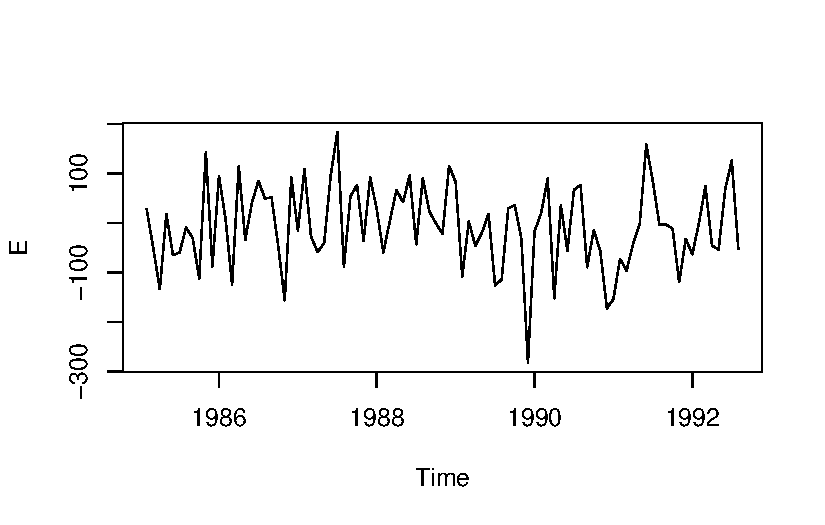
\includegraphics{Trabalhao1_ST_grupo5_2023_05_16_files/figure-pdf/unnamed-chunk-14-1.pdf}

}

\end{figure}

Agora observemos a análise visual dos resíduos.

\begin{Shaded}
\begin{Highlighting}[]
\FunctionTok{par}\NormalTok{(}\AttributeTok{mfrow=}\FunctionTok{c}\NormalTok{(}\DecValTok{1}\NormalTok{,}\DecValTok{3}\NormalTok{))}
\FunctionTok{plot}\NormalTok{(E)}
\FunctionTok{qqnorm}\NormalTok{(E); }\FunctionTok{qqline}\NormalTok{(E)}
\FunctionTok{acf}\NormalTok{(E, }\AttributeTok{lag.max=}\DecValTok{12}\SpecialCharTok{*}\DecValTok{5}\NormalTok{)}
\end{Highlighting}
\end{Shaded}

\begin{figure}[H]

{\centering 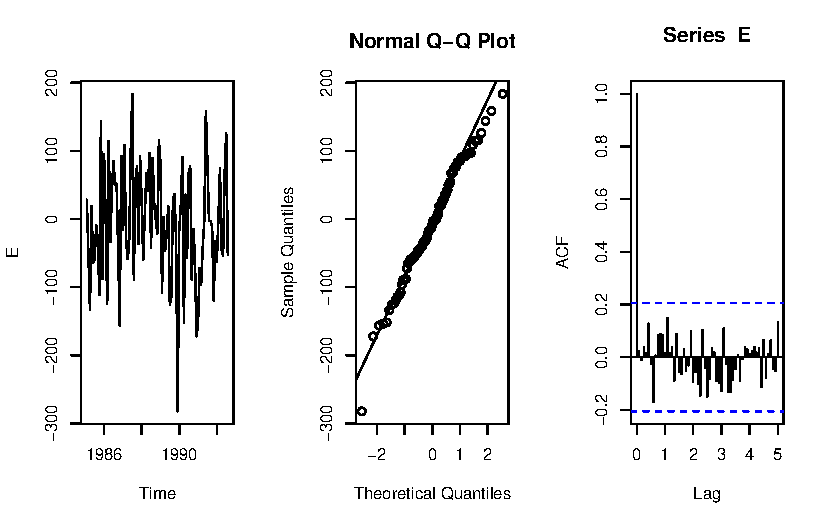
\includegraphics{Trabalhao1_ST_grupo5_2023_05_16_files/figure-pdf/unnamed-chunk-15-1.pdf}

}

\end{figure}

Os resíduos em si parecem estar estacionários (primeiro gráfico), já que
nenhuma tendência clara é observada, com os valores oscilando em torno
do zero. O quáfico QQplot, que compara os quantis esperados da normal e
os observados mostra que a distrubuição se comporta como uma
distribuição normal para a maior parte dos dados, mostrando apenas
alguns desvios nas caudas, principalmente à direita. Finalmente, o
gráfico ACF mostra a autocorrelação apenas para o primeiro valor, como
se espera, e não apresenta mais valores significativos de autocorrelação
a partir daí. Isso também indica que erros estão de fato se comportando
como um ruído branco.

Para completar essa análise, vamos proceder com alguns testes de
hipótese com significância de 5\%. O Teste de KPSS para verificar
estacionariedade , o teste de Ljung-Box para verificar se há
autocorrelação e finalmente o teste de Shapiro-WIlk para verificar se a
distribuição é compatível com a normal. Para todos esses testes
rejeitaríamos a Hipótese nula se o p-valor encontrado for \textless0.05.

A tabela abaixo mostra os resultados dos testes:

\begin{Shaded}
\begin{Highlighting}[]
\NormalTok{tabela2 }\OtherTok{\textless{}{-}} \FunctionTok{tibble}\NormalTok{(}
  \AttributeTok{estac =}\NormalTok{ tseries}\SpecialCharTok{::}\FunctionTok{kpss.test}\NormalTok{(E)}\SpecialCharTok{$}\NormalTok{p.value,}
  \AttributeTok{indep =} \FunctionTok{Box.test}\NormalTok{(E, }\AttributeTok{lag=}\DecValTok{15}\NormalTok{, }\AttributeTok{type =} \StringTok{"Ljung{-}Bo"}\NormalTok{)}\SpecialCharTok{$}\NormalTok{p.value,}
  \AttributeTok{normlt =} \FunctionTok{shapiro.test}\NormalTok{(E)}\SpecialCharTok{$}\NormalTok{p.value}

\NormalTok{)}
\NormalTok{tabela2 }\SpecialCharTok{\%\textgreater{}\%}
\NormalTok{  knitr}\SpecialCharTok{::}\FunctionTok{kable}\NormalTok{(}
    \AttributeTok{format =} \StringTok{"latex"}\NormalTok{,}
    \AttributeTok{align =} \StringTok{"c"}\NormalTok{,}
    \AttributeTok{booktabs =} \ConstantTok{TRUE}\NormalTok{,}
    \AttributeTok{longtable =} \ConstantTok{TRUE}\NormalTok{,}
    \AttributeTok{linesep =} \StringTok{""}\NormalTok{,}
    \AttributeTok{col.names =} \FunctionTok{c}\NormalTok{(}\StringTok{"Teste KPSS {-} estacionariedade"}\NormalTok{, }\StringTok{"Teste Box{-}Ljung {-} independência"}\NormalTok{, }\StringTok{"Teste Shapiro{-}Wilk {-} normalidade"}\NormalTok{),}
\NormalTok{    ) }\SpecialCharTok{\%\textgreater{}\%}
\NormalTok{  kableExtra}\SpecialCharTok{::}\FunctionTok{kable\_styling}\NormalTok{(}
      \AttributeTok{position =} \StringTok{"center"}\NormalTok{,}
      \AttributeTok{latex\_options =} \FunctionTok{c}\NormalTok{(}\StringTok{"striped"}\NormalTok{, }\StringTok{"repeat\_header"}\NormalTok{),}
      \AttributeTok{stripe\_color =} \StringTok{"gray!15"}\NormalTok{)}
\end{Highlighting}
\end{Shaded}

\begin{longtable}{ccc}
\toprule
Teste KPSS - estacionariedade & Teste Box-Ljung - independência & Teste Shapiro-Wilk - normalidade\\
\midrule
\endfirsthead
\multicolumn{3}{@{}l}{\textit{(continued)}}\\
\toprule
Teste KPSS - estacionariedade & Teste Box-Ljung - independência & Teste Shapiro-Wilk - normalidade\\
\midrule
\endhead

\endfoot
\bottomrule
\endlastfoot
\cellcolor{gray!15}{0.1} & \cellcolor{gray!15}{0.837631} & \cellcolor{gray!15}{0.5106649}\\*
\end{longtable}

O modelo ajustado cumpre os pré-requisitos de estacionariedade,
independencia e normalidade, indicando que é um moledo que pode explicar
a série.

\hypertarget{d.-apresente-a-equauxe7uxe3o-do-modelo-selecionado.}{%
\subsection{d.~Apresente a equação do modelo
selecionado.}\label{d.-apresente-a-equauxe7uxe3o-do-modelo-selecionado.}}

\begin{itemize}
\tightlist
\item
  Utilize a estimava dos parâmetros. Exemplo: o modelo selecionado é um
  SARIMA (0,1,2)(0,1,1) definido como
\end{itemize}

\begin{Shaded}
\begin{Highlighting}[]
\NormalTok{fit}\SpecialCharTok{$}\NormalTok{coef}
\end{Highlighting}
\end{Shaded}

\begin{verbatim}
       ma1        ma2       sma1 
-0.3468109  0.1799072 -0.7813321 
\end{verbatim}

Inicialmente vamos escrever o processo \(w_t\), após a diferenciação:

\(w_t = \nabla_s\nabla x_t = \nabla_s(x_t - x_{t-1}) = x_t - x_{t-12} - x_{t-1} - x_{t-11} , t > 13\)

Agora o processo \(w_t\) é um modelo ARIMA (0,0,2) x (0,0,1)

\(w_t =(1-0.78B^{12})(1 -0.35B + 0.18B^2)\epsilon_t\)

\hypertarget{e.-extra}{%
\subsection{e. Extra}\label{e.-extra}}

Apenas para efeito de comparação, ajustamos o modelo com a função
auto-arima. Essa solução apresentou ma pequena diferença do nosso
modelo, pois considerou a ordem da parte simples como um MA(3), enquanto
nós selecionamos um de ordem 2 para essa parte. Entretanto, como o nosso
modelo se ajusta bem, apresentando bom comportamento dos resíduos,
escolheríamos ele por ter menos parâmetros.

\begin{Shaded}
\begin{Highlighting}[]
\NormalTok{fit2 }\OtherTok{=} \FunctionTok{auto.arima}\NormalTok{(dados)}
\NormalTok{fit2}
\end{Highlighting}
\end{Shaded}

\begin{verbatim}
Series: dados 
ARIMA(0,1,3)(0,1,1)[12] 

Coefficients:
          ma1     ma2     ma3     sma1
      -0.3485  0.1070  0.1906  -0.7767
s.e.   0.1031  0.0992  0.1180   0.1222

sigma^2 = 7182:  log likelihood = -607.04
AIC=1224.07   AICc=1224.69   BIC=1237.24
\end{verbatim}

\hypertarget{e.-no-final-do-relatuxf3rio-inclua-como-um-apuxeandice-o-cuxf3digo-do-r-que-foi-utilizado.}{%
\subsection{e. No final do relatório, inclua como um apêndice o código
do R que foi
utilizado.}\label{e.-no-final-do-relatuxf3rio-inclua-como-um-apuxeandice-o-cuxf3digo-do-r-que-foi-utilizado.}}



\end{document}
